\newcommand{\CaseID}{circular_no_wind}
\newcommand{\CaseTitle}{Circular Spread Test (No Wind)}
\newcommand{\CaseOwner}{Cleo Lepart}
\newcommand{\CaseVersion}{v0.1}
\newcommand{\CaseDate}{\today}


\documentclass[../report/case_report.tex]{subfiles}

\begin{document}

\subsection*{Case Summary}

\textbf{Case ID:} \CaseID

\textbf{Objective:}
Verify that the ELMFIRE level-set solver produces isotropic fire spread when wind and terrain forcing are absent. Under homogeneous conditions the fire perimeter should expand radially, producing circular isochrones.

\subsection{Assumptions}

\begin{itemize}[nosep]
\item Homogeneous fuel model across the domain
\item Zero wind speed
\item Flat terrain (slope = 0)
\item Uniform fuel moisture
\item No spotting or suppression
\item Single ignition point
\end{itemize}

\subsection{Simulation Setup}

The computational domain is a square region with side length \SI{12}{km}.
The mesh resolution is \SI{30}{m}, producing a grid of 400×400 cells.

Meteorological and fuel parameters are spatially uniform and are generated using the preprocessing script derived from the ELMFIRE constant-wind tutorial.

\subsubsection{Input Data}

Input rasters represent constant fields:

\begin{itemize}
\item wind speed = 0
\item slope = 0
\item constant fuel model
\item constant moisture
\end{itemize}

\subsubsection{Numerical Controls}

\begin{itemize}
\item grid spacing $\Delta x = \Delta y = \SI{30}{m}$
\item timestep = \SI{30}{s}
\item simulation duration = \SI{21600}{s}
\end{itemize}

\subsection{Expected Results and Reasoning}

Under homogeneous fuel and zero wind, the rate of spread is isotropic.

The fire front therefore propagates radially from the ignition point.

\[
r(t) = R t
\]

where \(R\) is the constant rate of spread.

Isochrones should therefore form concentric circles centered at the ignition location.

\subsection{Acceptance Criteria}

\begin{itemize}
\item Isochrones appear circular
\item Radius increases linearly with time
\item Deviation from circular symmetry < 5\%
\end{itemize}

\subsection{Results}

The circular spread test evaluates whether the level-set propagation
produces isotropic fire growth when wind and slope are zero.

\begin{figure}[h]
\centering
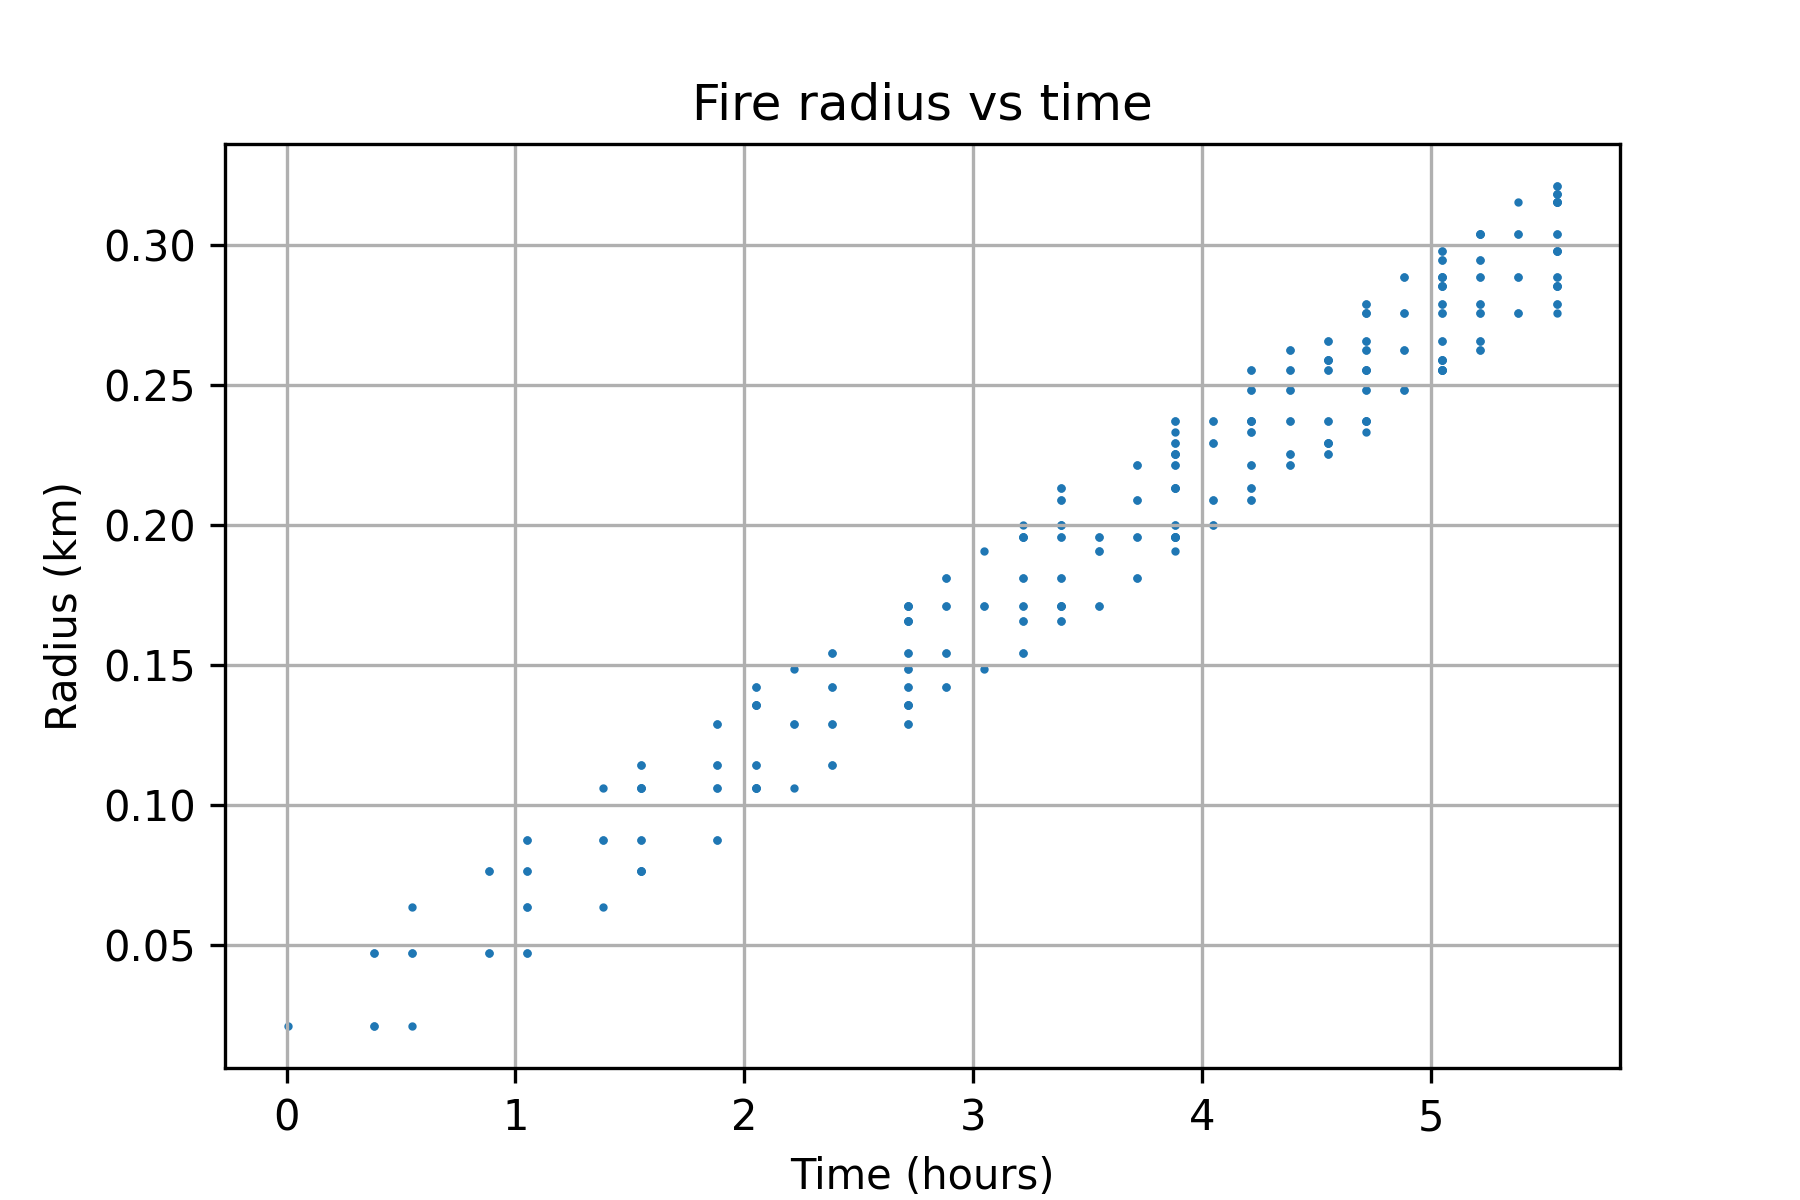
\includegraphics[width=0.7\textwidth]{figures/radius_vs_time.png}
\caption{Fire radius as a function of time computed from the
time-of-arrival raster. Linear growth indicates constant spread rate
and isotropic propagation.}
\end{figure}

\subsection{Discussion}

This case verifies that the ELMFIRE level-set solver produces isotropic fire spread when environmental forcing is absent.

\end{document}
